%!TEX root = main.tex

\section{Download connection analysis}
\label{sec:download-connection}

In this section, we will analysis the connection between the front-end server and the watch app. First we show the keep alive packets which are used to keep the connection alive. Then we analyis the different behavior between the image and voice frame in these TCP connections. And at last we try to figure out what factors influence the variety of RTT.

\subsection{Keep alive packets}
\label{sub:alive}

Keep alive pakcets in TCP have two main functions. One is to check whether the peer dead when when there are not packets to send for a while. The other one is to prevent disconnection due to network inactivity. Some middlebox, such as NAT and firewall may discard old and inactive connections deal to its finite memory, so sending keep alive packets may prevent deleting those alive connections which do not have data to send for a while. The personal live video system uses keep alive packets to keep the connections alive and the interval of sending keep alive packet is set as 5 seconds. Both the upload and download flows use keep-alive packets to keep the connections and that ensure consumers can send or receive packets even if the client does not send image or voice packet for a while. The server will terminate the flow if it does not receive acknowlagment of keep alive packet, nor it will continue to keep the flow alive. If a video provider breaks its connection and stops sending video for a while, the viewer will not receive video packets from the front-end server but still sending keep alive packets to keep the connection alive. When the same video provider sets up another connection to send video to the front-end server, the server will continue to send vieo to the viewer using the alive connection. Table~\ref{tbl:alive-packet} shows the percentage of keep alive packets' number and time. From the table we can see that the keep alive time consists of 10.1\% of all download flow's flow complete time, while 2.5\% for upload flow. That means viewers spend about 10\% of their view time to wait when the providers terminate to send their video. The upload flow also has 2.5\% keep alive time that the front-end server sends keep alive packets to the camera if it has not received vedio for a while. 

\begin{table}[ht]
\tablefontsize
\renewcommand{\arraystretch}{\assize}
 \setlength{\tabcolsep}{3pt}
\caption{Percentage of keep alive packets.}
\centering
\begin{tabular}{c|c|c}
	\toprule
	 flow type & keep alive packet number & keep alive time \\
	\hline
	download flow & 7.3\% & 10.1\% \\
	\hline
	upload flow & 5.9\% & 2.5\% \\
	\bottomrule
\end{tabular}
\label{tbl:alive-packet}
\termspace
\end{table}  

\subsection{Different behavior of image frame and voice frame}
\label{sub:diff-gra-voice}

A video TCP connection consists of two main frame: image frame and voice frame. The size of image frame is 3K-20K bytes, much larger than the voice frame which is about 400 bytes. Each TCP connection has its own MSS(Maximum Segment Size) which is equal as MTU(Maximum Transmission Unit). The MTU of Ethernet is 1460 bytes, so a image frame will be divided into several TCP packets. That means image frame often result in a burst of packet into network, while voice frame just one small packet into the network. Such different behavior of the two frame will result in defferent effect in the network. We will further detail the different effects of the two frames in network.

%As the image frame is often divided into several TCP packets, it is easier to produce burst compare to the voice frame. Figure~\ref{fig:burst-packet} shows the different number of burst packets for the two frames. From the figure we can see that for image frame over 25\% burst has 2 packets and over 10\% has 4 packets. For voice frame only 10\% burst is larger than 2 packets and only 2\% burst is larger than 4 packets. Image frame's large burst packet number will make it easier to loss packet.

%\begin{figure}[ht]
%	\centering
%	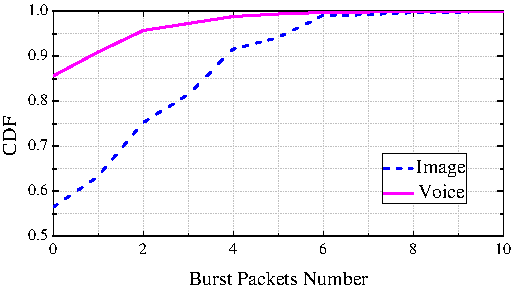
\includegraphics[width=\linewidth]{burst-packet}
%	\caption{Different number of burst packet for image and voice frame.}
%	\label{fig:burst-packet}
%	\termspace
%\end{figure}

Table~\ref{tbl:loss-timeout-rate} shows the different loss rate and time out retransmission rate of different frame. From the table we can see that the total packets' loss rate is 0.61\%.  The image frame's loss rate is 0.76\%, higher than the voice frame which is only 0.33\%. We believe the higher loss rate is caused by the two different behaviors of image frame and voice frame. One is the burst feature of image frame, shown in Figure~\ref{fig:burst-packet}. The other is that the TCP packets of image frame are larger than voice packets, and routers trend to drop the larger packet. However we find that for voice frame the timeout retransmission rate among loss packets are much higher than image frame. For voice frame, 31.6\% of the loss packets are recovered by timeout retransmision while others are recovered by fast retransmission. For image frame 20.7\% of the loss packets are recovered by timeout retransmision. We will detail different type of timeout retransmision to illustrate why this happen. 

\begin{table}[ht]
\tablefontsize
\renewcommand{\arraystretch}{\assize}
 \setlength{\tabcolsep}{3pt}
\caption{The different loss and timeout retransmission rate.}
\centering
\begin{tabular}{c|c|c}
	\toprule
	 frame type & packet loss  &  timeout retrans./loss \\
	\hline
	image frame & 0.76\%  & 20.7\% \\
	\hline
	voice frame & 0.33\% & 31.6\% \\
	\hline
	total & 0.61\%  & 22.7\% \\
	\bottomrule
\end{tabular}
\label{tbl:loss-timeout-rate}
\termspace
\end{table}  

%If the fast retransmit can not recovered a lost packet, it has to trigger timeout retransmission. According the situation when the timeout retransmssion happens, the timeout retransmission can be divided into several types. If the fast retransmit packet is drop by the network, timeout retransmission has to be triggered and we refer this timeout retransmission as double retrans. If the lost packet is the last three packets of the flow, there are not enough duplicate acknowledgments (dupacks), referred to as tail retransmission. Less dupacks to trigger fast retransmit may also deal to the server send less than 4 packets out(either because there are not enough packets or the cwnd is small), and we refer it as less pkt retransmission. The ACK delay/loss or all of the packets send out lost will also result in timeout retransmission, as at both of the two situations no dupacks can be produced. We refer the two timeout retransmissions as  ACK delay/loss and continuous loss respectively. 

%Table~\ref{tbl:time-out-type} shows the time of each timeout retransmission in both of the image and voice frame. Those that cannot be classified into any of the above type of timeout retransmission is reffered to as others. From the table we can see that less pkt retransmission contributes the largest part (i.e.,56.2\%) for voice frame, much higher than the image frame(i.e.,36.9\%). As the voice frame is less than one MSS, when sending the voice frame, there are often few packets in the network compared with sending image frame. That not only explains why less pkt retransmission is much higher for voice frame, but also shed light on voice frame's high timeout retransmissin rate in Table~\ref{tbl:loss-timeout-rate}. In Table~\ref{tbl:loss-timeout-rate} the voice frame has smaller packet loss rate but higher timeout retransmissin rate. For image frame, the higher packet loss rate results in higher double retrans, ACK delay/loss and continuous loss. As the voice frame seldom send out at the tail of flow, the fraction of tail retransmission is much smaller for the voice frame.   

%\begin{table}[ht]
%\tablefontsize
%\renewcommand{\arraystretch}{\assize}
% \setlength{\tabcolsep}{3pt}
%\caption{The time of different type of timeout retransmission.}
%\centering
%\begin{tabular}{c|c|c}
%	\toprule
%	 timeout retransmission type & image frame & voice frame \\
%	\hline
%	tail retrans. & 2.8\% & 0.2\% \\
%	\hline
%	less pkt retrans. & 36.9\% & 56.2\% \\
%	\hline
%	double retrans. & 28.7\% & 24.6\% \\
%	\hline
%	ACK delay/loss & 13.2\% & 8.7\% \\
%	\hline
%	continuous loss & 2.7\% & 0 \\
%	\hline
%	others & 15.8\% & 10.3\% \\
%	\bottomrule
%\end{tabular}
%\label{tbl:time-out-type}
%\termspace
%\end{table}  

\subsection{Varity of RTT}
\label{sub:RTT}

RTT is an important factor that influence the flow rate. The flows with smaller RTT are more likely to get high flow rate. RTT is determined by two factors. One is number of hops between two nodes which is controlled by the route algorithm. The other is the packets' cache time at the routers which is controlled both by the router buffer capacity and the volume of packets in the network. In the WAN(Wide Area Network), the route algorithm and router buffer capacity is out of the control of sever. The only way that the server can control the RTT is by controlling the packets that is sent to the network.

In table~\ref{tbl:inflight-rtt} we analysis the change of RTT when the $in\_flight$ change. $in\_flight$ is the number of packet in flight which is defined as the following equation:

\begin{footnotesize}
 \begin{equation}
\label{eq:conserve}
\begin{aligned}
in\_flight = \enspace & packets\_out + retrans\_out \enspace - \\
& (sacked\_out + lost\_out) \enspace ,
\end{aligned}
\end{equation}
\end{footnotesize}

where $packets\_out$ is the number of packets between $snd\_una$ (the packet with highest sequence number the receiver has acknowledged) and $snd\_nxt$ (the next new segment the sender would transmit), $retrans\_out$ is the number of retransmitted but not yet acknowledged packets, $sacked\_out$ is the number of SACKed packets, and $lost\_out$ is the number of lost packets.

We examine the change of RTT as we compare it with the RTT which is calculated in the 3-way handshake(3WHS) phase(referred to as 3WHS\_RTT). From table~\ref{tbl:inflight-rtt} we can see that as the $in\_flight$ become large, the RTT grows compared with the 3WHS\_RTT. When the $in\_flight$ becomes as large as 64KB, the RTT is even 2.6 times of the 3WHS\_RTT. That means the RTT becomes large when the $in\_flight$ become large as the routers need more time to deal with the coming packets.      

\begin{table}[ht]
\tablefontsize
\renewcommand{\arraystretch}{\assize}
 \setlength{\tabcolsep}{3pt}
\caption{The varity of RTT when the $in\_flight$ packets changes.}
\centering
\begin{tabular}{c|c}
	\toprule
	 $in\_flight$ & RTT/3WHS\_RTT \\
	\hline
	$<$4KB & 0.89 \\
	\hline
	4KB-8KB & 1.08  \\
	\hline
	8KB-16KB & 1.31  \\
	\hline
	16KB-32KB & 1.38  \\
	\hline
	32KB-64KB & 1.61 \\
	\hline
	$>$64KB & 2.6  \\
	\bottomrule
\end{tabular}
\label{tbl:inflight-rtt}
\termspace
\end{table}  



